\section{General introduction}

\section{Macromolecular Crystallography}

\subsection{X-ray scattering}

X-rays are high energy photons part of the electromagnetic spectrum with a wavelength 0.1-10nm \cite{Rupp2010-nc}. X-rays can be described as packets of travelling electromagnetic waves, whose electric field vector interacts with the charged electrons of matter \cite{Rupp2010-nc}. Such interaction, typically termed scattering, results in the diffraction of the incoming wave, which X-ray crystallography relies on.

In its simplest form, scattering of X-ray radiation can be explained in the scenario of exposure to a single free electron. The resulting scattering can be classed as elastic (Thomson scattering) or inelastic (Crompton scattering) \cite{Rupp2010-nc}. The latter --- scattering that results in a loss of energy of the emitting photon due to energy transfer onto the electron --- does not contribute to discrete scattering, the type of scattering X-ray diffraction relies on. In comparison, Thomson scattering does not result in a loss of energy of the emitting photon. This has significant effects, the incoming photon emits with the same frequency causing the electron to oscillate identically further enhancing the signal. However, it is important to understand that the scattering function of an electron is non-isotropic since the scattered intensity emits strongest in forward and backward directions \cite{Rupp2010-nc}.

If we expand the example to include all electrons in an atom and expose the atom to X-ray radiation, our theory needs to be slightly expanded. Given thatone or more electrons in an atom are not free but orbit around the atom's nucleus in a stable and defined manner, the distribution of these electrons around the nucleus determines the scattering of the incoming X-ray photons. The distribution of scattered photon waves is thus an overall representation of the probability distributions of each electron in the atom and is refered to as electron density $\rho(\boldsymbol{r})$. In X-ray scattering, it suffices to approximate the shape of the electron density to a sphere. If we now consider the emitting wave $\boldsymbol{s_1}$ of an X-ray photon scattered by any position $\boldsymbol{r}$ in the electron density of an atom, then the phase difference $\Delta\varphi$ to the incoming wave $\boldsymbol{s_0}$ can be described by \cref{eq:phase_difference} \cite{Rupp2010-nc}. 

\begin{equation}
    \Delta\varphi=2\pi\left(\boldsymbol{s_1}-\boldsymbol{s_0}\right)\boldsymbol{r}=2\pi \cdot \boldsymbol{S}\boldsymbol{r}
    \label{eq:phase_difference}
\end{equation}

If more than one electron in an atom's electron density scatter the incoming X-ray wave, then the emitting partial waves can be described by the atomic scattering function $f_s$ (\cref{eq:atomic_scattering_factor}), which describes the interference of all scattered waves \cite{Rupp2010-nc}. The total scattering power of an atom is proportional to the number of electrons and element-specific with heavier atoms scattering more strongly. Given the approximation of a centrosymmetric electron density, the atomic scattering function is also symmetric. 

\begin{equation}
    f_s=\int\limits_{\boldsymbol{r}}^{V(atoms)}\rho\left(\boldsymbol{r}\right) \cdot e^{2\pi\\i\boldsymbol{S}\boldsymbol{r}} \cdot d\boldsymbol{r}
    \label{eq:atomic_scattering_factor}
\end{equation}

With an enhanced understanding of X-ray scattering of electrons orbiting a single atom, it is important to consider X-ray scattering of adjacent atoms, such as it is typically found in molecules. If the electromagnetic wave of a X-ray photon excites all electrons of adjacent atoms, then the resulting partial waves result in constructive or destructive interference. Maximal interference can be obtained when all partial waves are in phase, and maximal destructive interference when out-of-phase. This leads to varying intensities of the emitting X-ray photon at different points in space. To obtain the overall scattering power $F_s$ of all contributing atoms, \cref{eq:atomic_scattering_factor} needs to be modified to include the sum over all atoms $j$ as described in \cref{eq:total_scattering_power}.

\begin{equation}
    F_s=\sum_{j=1}^{atoms}f_{s,j}^0 \cdot e^{2\pi\\i\boldsymbol{S}\boldsymbol{r}_j}
    \label{eq:total_scattering_power}
\end{equation}

If we now translate our hypothetical experiment into a crystal lattice then our understanding described in \cref{eq:total_scattering_power} needs to be expanded from a 1-dimensional distance vector $\boldsymbol{r}$ to the three dimensional lattice translation vectors $\boldsymbol{a}$, $\boldsymbol{b}$ and $\boldsymbol{c}$. The Laue equations (\cref{eq:laue_equations}) do exactly that and ultimately determine the positions of the diffraction peaks in 3-dimensional space.

\begin{equation}
    \boldsymbol{S} \cdot \boldsymbol{a}=n_1, \quad \quad \boldsymbol{S} \cdot \boldsymbol{b}=n_2, \quad \quad \boldsymbol{S} \cdot \boldsymbol{c}=n_3
    \label{eq:laue_equations}
\end{equation}

\begin{equation}
    n\lambda=2d_{hkl}sin\theta
    \label{eq:bragg_equation}
\end{equation}

Such determination is possible through the findings made by \textcite{Bragg1913-cx}, who identified the relationship between the scattering vector $\boldsymbol{S}$ and the planes in the crystal lattice. Today, this relationship is defined by the Bragg equation (\cref{eq:bragg_equation}) \cite{Bragg1913-cx}, which allows us to interpret X-ray diffraction as reflections on discrete lattice planes, which relates the diffraction angle $\theta$ to the lattice spacing $d_{hkl}$ (\cref{fig:introduction_bragg}) \cite{Rupp2010-nc}. For maximum diffraction $n$ needs to be integer multiples to result in maximum constructive interference of wavelength $\lambda$.

\begin{figure}[H]
    \centering
    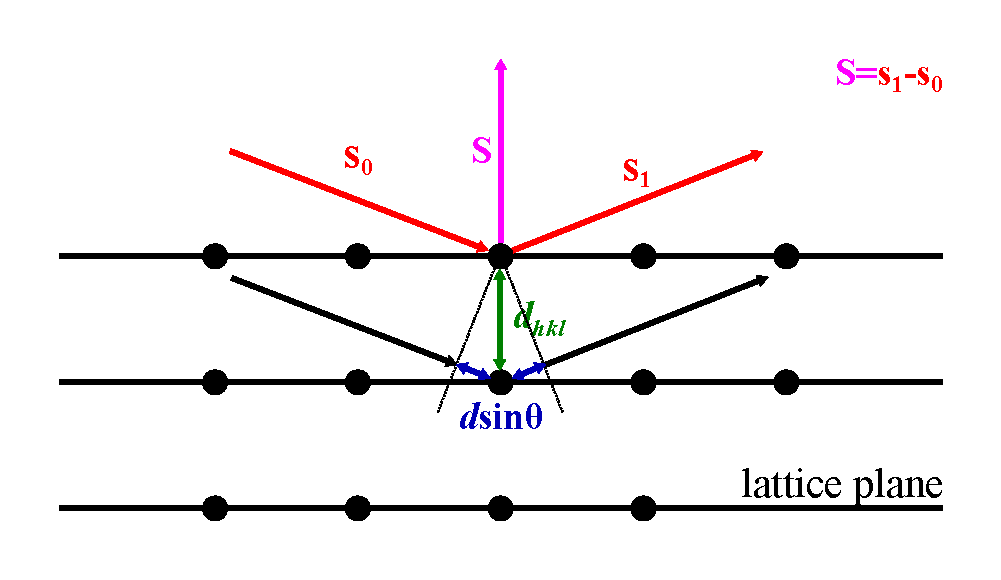
\includegraphics[width=\textwidth]{introduction_bragg.pdf}
    \caption{Schematic of Bragg scattering.}
    \label{fig:introduction_bragg}
\end{figure}

Lastly, if the hypothetical model is expanded to molecular crystals, then the total scattering from the unit cell is merely a summation of all molecular unit cell scattering contributions in the crystal. Mathematically, this results in \cref{eq:total_scattering_power} being generalised to \cref{eq:structure_factors} through the application of the Laue equations (\cref{eq:laue_equations}) to express the scattering vector $\boldsymbol{S}\boldsymbol{r}_j$ as Miller indices of the reflection planes $\boldsymbol{h}\boldsymbol{x}_j$. 

\begin{equation}
    F_h=\sum_{j=1}^{atoms}f_{s,j}^0 \cdot e^{2\pi\\i\boldsymbol{h}\boldsymbol{x}_j}
    \label{eq:structure_factors}
\end{equation}

The structure factor equation defines the scattering power from a crystal in a given reciprocal lattice direction $\boldsymbol{h}$. The scattering is enhanced by the number of repeating units of lattice translation vectors $\boldsymbol{a}$, $\boldsymbol{b}$ and $\boldsymbol{c}$, and thus the overall scattering power is proportional to the number of unit cells in the crystal.

It should be noted that \cref{eq:structure_factors} is a simplification of the problem at hand. In reality, instrument and experimental corrections need to be applied to the structure factor equation. A correction factor for each experiment-dependent parameter needs to be applied to the structure factor equation. However, in the scope of this work the details of such correction factors do not need to be discussed.

\begin{equation}
    \rho(x,y,z)=\frac{1}{V}\sum_{h=0}^{+\infty}\sum_{k=-\infty}^{+\infty}\sum_{l=-\infty}^{+\infty}\boldsymbol{F}(hkl)\cdot e^{-2\pi\\i(hx+ky+lz)}
    \label{eq:electron_density}
\end{equation}

Since complex structure factors describe the molecular structure in the reciprocal space domain, the conversion to the real space domain in form of electron density is required. This can be conveniently done through the bijective Fourier transform, which allows to convert complex structure factors to electron density and vice versa without the loss of any information \cite{Rupp2010-nc}. Thus, electron density can be obtained from the complex structure factors using \cref{eq:electron_density}. The normalisation factor $1/V$ provides the correct units for the electron density $\rho(x,y,z)$.

\subsection{Structure determination}

